% In this section we present building blocks for an optically implemented CNN. In this rest of this paper we focus on the convolutional layer, but we will briefly discuss other layers here too.

% \paragraph{CNN architecture variations} Our goal is to match performance with a constrained optical setup, so also relevant to highlight are CNNs with non-standard architectures that may align with physical designs. Omission of fully connected layers, i.e. fully convolutional with global average pooling at the top layer has proven to be successful in \cite{lin2013network,iandola2016squeezenet}. Analysis of CNN operations in the Fourier domain, introducing spectral pooling and regularization \cite{rippel2015spectral}. Relevant because we can also access optical Fourier plane. We also note the work in the complex-valued deep neural networks \cite{trabelsi2017deep}, as coherent optical signals may be an effective means of propagating complex-valued data.

In this section we describe proposed optical building blocks corresponding to common layers in a CNN. We only consider standard feed-forward CNNs, where information is passed in a single direction through a sequence of layers. Cycles, loops, interacting networks, and other more complicated architectures could be interesting to explore in the future. For now, we will focus on the most essential components that define a CNN in the context of an image classification task. Later, these building blocks will be used to simulate classification models consisting of a single optical convolutional layer (i.e. an optical correlator), one optical convolutional layer fed into one digital fully connected layer, and a fully optical convolutional neural network. Note that we assume spatially incoherent light as the input to the proposed systems as this is most relevant to an imaging scenario.

\subsection*{Convolutional layer}

\begin{figure}[t]
\centering
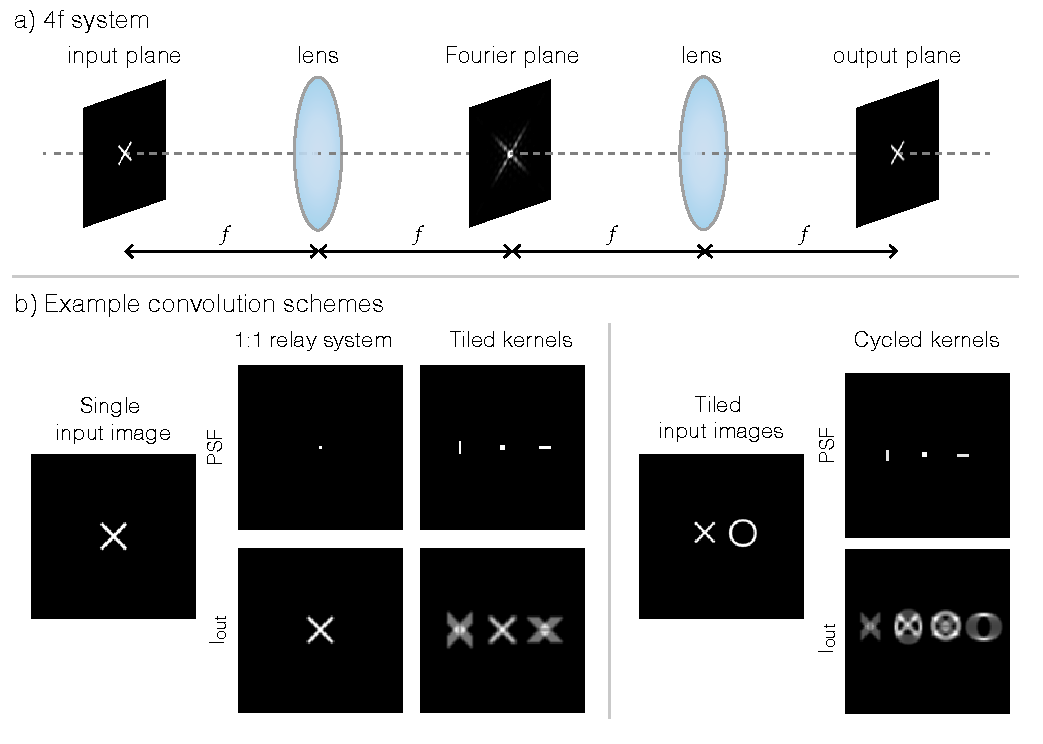
\includegraphics[width=\linewidth]{convolution.pdf}
\caption{Optical convolutional layer}
\label{fig:convolution}
\end{figure}

A CNN typically begins with a convolutional layer, which essentially performs pattern matching with a set of learnable visual filters. A standard convolutional layer takes an input volume of depth $C_\text{in}$, performs a series of correlations with a set of $C_\text{out}$ kernels each with depth $C_\text{in}$, and outputs a new volume of depth $C_\text{out}$. The correlation of the kernel across the width and height of the input volume produces a 2D ``activation map", and stacking the $C_\text{out}$ activation maps for all kernels forms the output volume of depth $C_\text{out}$. Hyperparameters include the spatial extent of the kernel $F$, the stride with which the kernel is applied, and the padding of the input volume. Here we assume a stride of $1$, meaning the kernel is shifted by one pixel at a time, and zero-padding such that the output volume has the same height and width as the input. Each channel of the output image from a single non-strided, zero-padded convolutional layer can be described as:
\begin{equation}
I_\text{out, j}  = \sum_{i = 1}^{C_\text{in}} I_\text{in, i} \ \star \ \text{W}_{i,j}\ , \text{for } j \in 1, 2, \hdots C_\text{out} 
\end{equation}

In linear optical systems, image formation is often modeled as a spatially invariant convolution of the scene with the point spread function (PSF) of the system:
\begin{equation}
I_\text{out}  = I_\text{in} * \text{PSF}
\end{equation}

One way to achieve this setup is with a ``4$f$ system", a basic telescope consisting of two convex lenses performing a cascade of two Fourier transforms (Fig. \ref{fig:convolution}a). The system is so-named due to the placing of the first lens one focal distance, $f$, away from the object plane, producing a Fourier plane another distance $f$ in front of the first lens. The second lens is then placed another distance $f$ from the Fourier plane, producing a conjugate image plane a final distance $4f$ from the original object plane \ref{fig:convolution}. The Fourier plane of such a system can be modulated in amplitude and phase, akin to a bandpass filter in signal processing, which alters the PSF of the system \cite{goodman2008introduction}.  This simple case can be viewed as a convolutional layer with $C_\text{in} = C_\text{out} = 1$ and the flipped PSF as the single kernel. We will also refer to the flipped PSF as the kernel since the flipping is trivial. 

\subsubsection*{Tiled kernels} Now suppose we want $C_\text{out} = n$ where $n >1$. By spatially tiling the multiple kernels as the PSF of the system in an $A \times B$ grid, the output becomes the convolution of the input image with multiple 2D kernels, but now the $n$ outputs are tiled laterally instead of stacked in depth. Consideration can be taken to ensure these outputs are non-overlapping by adjusting the shifts $\Delta x$ and $\Delta y$, if desired. The PSF can be described as
\begin{equation}
{PSF}(x,y) = \sum_{a = 1}^{A}\sum_{b = 1}^{B} W_{aB+b} (x,y) * \delta(x - a\Delta x, y - b\Delta y),
\end{equation}
and the resulting image formation as
\begin{equation}
I_\text{out}(x,y) = [I_\text{in} * PSF](x,y) =\sum_{a = 1}^{A}\sum_{b = 1}^{B}  [I_\text{in} * W_i](x) * \delta(x - a\Delta x, y - b \Delta y)
\end{equation}
where $W$ corresponds to a standard multichannel kernel for a single channel input image. Hence we have a way to convolve a single input image with multiple 2D kernels, with the difference here being that the multiple output channels are tiled across the 2D image plane instead of stacked in a third ``depth" dimension.

\subsubsection*{Cycled kernels}
The next important extension is to incorporate $C_\text{in} = m$ where $m > 1$. If we needed to exactly imitate the digital CNN, we would need $m$ different kernels for each of the $m$ input channels. This could potentially be implemented with many of the single channel modules in parallel, with the addition of a relay that sums $m$ outputs that correspond to the different depth slices of the same kernel, but this type of setup may be prohibitively complicated to build. If we slightly relax our requirements, we could again rely on Fourier optics to perform the summation. Now suppose we have tiled input images in addition to the kernels, simplifying to 1D for now for clarity:
\begin{equation} I_\text{in}(x) = \sum_{j = 1}^m I_j(x)  * \delta(x - j\Delta x),\  PSF(x) = \sum_{i = 1}^m W_i(x)  * \delta(x - i\Delta x)\end{equation}

\begin{align} I_\text{out} &= [I_\text{in} * PSF](x)= \sum_{i=1}^n [I_\text{in} * W_i](x) * \delta(x - i\Delta x)  \\
&= \sum_{i=1}^n \sum_{j=1}^m\left( [I_\text{j} *  W_i](x) * \delta(x - j\Delta x) \right) * \delta(x - i\Delta x) 
\end{align}
This combination of tiled images and tiled kernels results in some cycling of the kernels, but could still potentially offer enough degrees of freedom for certain tasks. Examples of tiled kernels and cycled kernels are shown in Fig. \ref{fig:convolution}b.

\subsubsection*{Large PSFs} Finally, we were curious whether we even needed to think about tiling many small kernels, or rather if we could optimize for one large PSF, and leave it to the optimization to decide whether tiling was the optimal strategy. These approaches are compared in later simulations.

\subsection*{Nonlinear activation layer}
In this paper, we primarily focus on the convolutional layers and apply nonlinear activations in simulations, when they used. However, we review some possible optically addressed approaches for the benefit of further research in this area, which also informs us on what type of activation functions to apply in simulation. 

Nonlinear activation layers are crucial components in the neural network toolbox that allow for modeling of nonlinear relationships between input and output variables. Most commonly used is a rectified linear unit (ReLU), that simply sets all negative values to 0: $\text{ReLU}(x) = \max\{0, x\}$. In an optical intensity-based system, there are no non-negative values, so the standard ReLU function does not directly apply. However, if we consider the purpose of the ReLU layer to zero out some fraction of the neurons below a threshold response level, then we hypothesize that we can accomplish a similar effect by shifting this threshold to a positive value. 

This nonlinear behavior translates to an ideal optical element that is fully opaque when incident light is low intensity and fully transmissive when incident light is above a threshold. A perfectly binary switch is difficult to physically realize, so instead we sought a material that would be less transmissive to lower incident intensities and become more transmissive at higher incident intensities. In fact, this type of nonlinear response is remniscent of the PReLU (parametrized ReLU) \cite{he2015delving} and (Swish) \cite{ramachandran2017searching}, only centered at a positive threshold instead of zero.

Bacteriorhodopsin (BR) is a membrane protein found in the bacterium \textit{Halobacterium salinarium} that has been shown to exhibit logarithmic transmittance at one of its absorbance peaks of $\sim$570 nm \cite{downie1995nonlinear}. The BR protein reversibly cycles between two states with the absorption of light, causing the appearance of a BR film to change from a deep purple to a light transparent purple. Furthermore, the shape of the transmittance function can be tuned by adjusting the concentration and pH of the BR solution before creation of the film \cite{thoma1991bacteriorhodopsin}. Besides BR, visible light-responsive DASA-polymer conjugates have been synthesized that also demonstrate reversible tunable absorption properties dependent on incident light intensity \cite{ulrich2017visible}. This compound shows more of a linear transmittance function, becoming more transparent with higher intensity light \cite{dolinski2017versatile}. We consider these in simulation to assess if a film or gel of these or similar substances could be used as a nonlinear activation layer in an ONN. 

\subsection*{Fully-connected layer}
The fully connected layer is so named because every input neuron is connected to every output neuron.
The output of the previous layer is flattened into a single vector and multiplied with a matrix of size $D_\text{out} \times D_\text{in}$, where $D_\text{in} = H\text{in} \times W\text{in} \times C_\text{in}$. For a limited size of $D_\text{out}$, this elementwise product could be implemented by splitting the input image into $D_\text{out}$ copies and performing an elementwise matrix multiplication using an amplitude mask. Unfortunately, this strategy becomes unreasonable as $D_\text{out}$ grows. 

Fortunately, fully connected layers may not be necessary, as fully convolutional networks have been successful in several prominent cases \cite{lin2013network,iandola2016squeezenet}. For example, if the goal is to classify among $Z$ classes, it is possible to end with a convolutional layer that produces an output with $Z$ channels, and then average each of the $Z$ channels to produce a score for each of the classes. This suggests we may be able to implement a series of optical convolutional layers, divide the final output image into $Z$ subregions, and then take the mean of each of those subregions.

\subsection*{Pooling layer}
Pooling layers can be inserted, commonly between convolutional layers, to reduce spatial size and consequently computation. Pooling operations, for example "maximum", operate on each depth slice independently. One of the main reasons for pooling is to reduce the computing needs by reducing the dimensions of the next input image, which we do not need to consider in an optical system. Otherwise, pooling may improve training and prevent overfitting.

While it is not obvious how to take the spatial maximum of an optical signal without active sensing, average pooling can be approximated with a reduction in the spatial resolution of the image. This can be accomplished with a low-pass filter, i.e. a small iris placed in the pupil plane of the last $4f$ system. Spectral pooling is another interesting concept used in spectral representations of CNNs that carries over easily to our ONN setup \cite{rippel2015spectral}. Spectral pooling can be viewed as a generalization of low-pass filter pooling, in particular allowing for specific bandwidths to be selected for using custom amplitude masks. We only mention pooling layers here but do not explore these in our further experiments, as they were not essential for our analysis of convolutional layers.

